\documentclass[12pt,a4paper]{article}
\usepackage[left=20mm,top=20mm,bottom=30mm]{geometry}
\usepackage{graphicx}

\begin{document}
\title{SkyHiGH Feide}
\author{Fredrik Magnussen, Håkon Tvedt og Morten Hanssen Singstad}
\maketitle 
\begin{center}
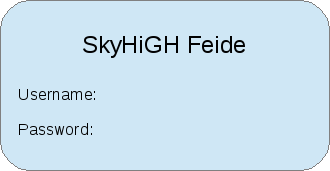
\includegraphics[scale=1]{frontpageimage.png}
\end{center}

\newpage
\tableofcontents


\newpage
\section{Forord}
Noe som fanget opp oppmerksomheten våres fra starten av, var utstyret vi skulle få sette opp og leke med. Den var ekstra attraktiv siden den er veldig relevant i henhold til driftstudie vi går, siden det ikke var så mange bacheloroppgaver som passet godt for nettverksdriftere i år. SkyHiGH Feide-oppgaven er etterfølger de tidligere SkyHiGH-oppgavene. Det som vi synes er spennende ved dette prosjektet, er at når vi er ferdig, så skal dette server-racket være oppe å kjøre og bli brukt. Den skal være høgskolens egen vm-server. Det er noe vi synes er veldig spennende.

\section{Insperation}
Let's see what happens when i do this.

\end{document}